\documentclass[tikz,border=6pt]{standalone}
\usepackage{amsmath,amssymb}
\begin{document}
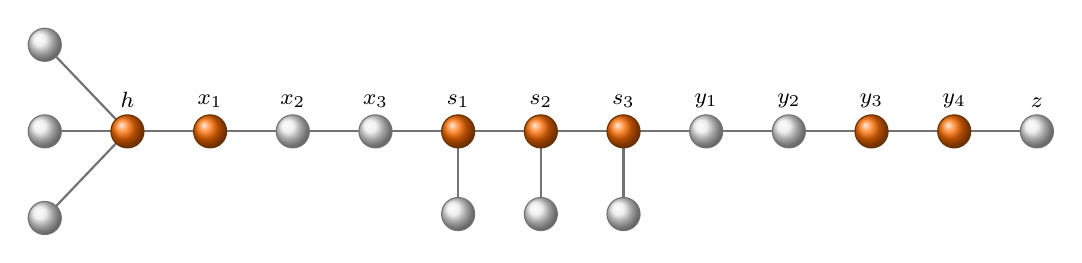
\begin{tikzpicture}[x=1.05cm,y=1cm,
  v/.style={circle,shading=ball,ball color=white!92!black,draw=black!55,minimum size=4.2mm,inner sep=0pt},
  d/.style={v,ball color=orange!85!red,draw=orange!40!black},
  e/.style={draw=black!55,line width=0.8pt},
  lab/.style={font=\footnotesize,inner sep=1pt}]
  % spine: h x1 x2 x3 s1 s2 s3 y1 y2 y3 y4 z
  \foreach \name/\xx in {h/0,x1/1,x2/2,x3/3,s1/4,s2/5,s3/6,y1/7,y2/8,y3/9,y4/10,z/11}
    \coordinate (\name) at (\xx,0);
  \foreach \k in {1,2,3} \coordinate (hl\k) at (-1.0,{1.1-1.1*(\k-1)});
  \foreach \k in {1,2,3} \coordinate (sl\k) at ({3+\k},-1.05);
  \draw[e] (h)--(x1)--(x2)--(x3)--(s1)--(s2)--(s3)--(y1)--(y2)--(y3)--(y4)--(z);
  \foreach \k in {1,2,3} { \draw[e] (h)--(hl\k); \draw[e] (s\k)--(sl\k); }
  % vertices; the total dominating set of size 7 is shaded
  \foreach \p in {x2,x3,y1,y2,z,hl1,hl2,hl3,sl1,sl2,sl3} \node[v] at (\p) {};
  \foreach \p in {h,x1,s1,s2,s3,y3,y4} \node[d] at (\p) {};
  % labels
  \node[lab,above=2.6mm] at (h) {$h$};
  \foreach \k in {1,2,3} \node[lab,above=2.6mm] at (x\k) {$x_{\k}$};
  \foreach \k in {1,2,3} \node[lab,above=2.6mm] at (s\k) {$s_{\k}$};
  \foreach \k in {1,2,3,4} \node[lab,above=2.6mm] at (y\k) {$y_{\k}$};
  \node[lab,above=2.6mm] at (z) {$z$};
\end{tikzpicture}
\end{document}
